\section{Electronic Mechanism of Mg Corrosion Inhibition}

In general, chemisorption on a transition metal surface is determined by two factors: a potential attractive energy term ($E_{attractive}$) related to the d-band center location relative to the Fermi level (i.e. so-called d-band center model), and a repulsive energy term ($E_{repulsive}$) related to the orbital overlap between the adsorbate orbital and the orbitals of other surface atoms (so-called Pauli repulsion) \cite{hammer1995electronic,hammer1995gold}:
\begin{align}
 %(9)
E_{chem adsorption} \sim E_{attractive} + E_{repulsive}
\label{Chap:Mg_H:eq:electronic}
\end{align}

We found that the effect of each of the 6 p-block elements identified as Mg corrosion inhibitors in Section 3c is negligible on the d-band center of Fe surface atoms. This was confirmed by computing and examining electronic density-of-states (Section S1 of the Supplementary Materials). Specifically, when one Fe atom in the top surface layer of (2$\times$2) Fe (100) or (110) was substituted by an alloying atom from one of 6 p-block elements, the change of d-band center for all atoms in the top surface layer was always less than 0.2 eV. According to previous DFT studies of a series of transition metals, a change of $\sim$1 eV in the d-band center of their surface atoms results in a change of $\sim$0.5 eV in H adsorption energy \cite{greeley2006computational}. Thus, it is not expected that such small changes in the d-band center for an Fe surface with p-block substitutional elements reported here can induce significant variations of hydrogen adsorption strengths.

\newpage
\begingroup
\begin{figure}[!ht]
  \centering
  \subfigure[]{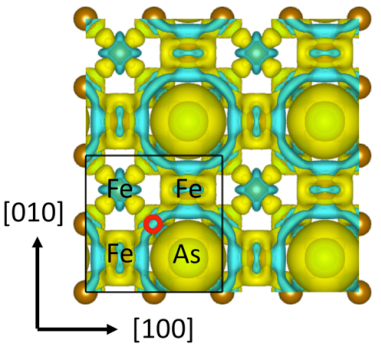
\includegraphics[width=0.45\linewidth]{Chap3/plots/Fig10a.pdf}}\label{Chap:Mg_H:fig:10a}
  \subfigure[]{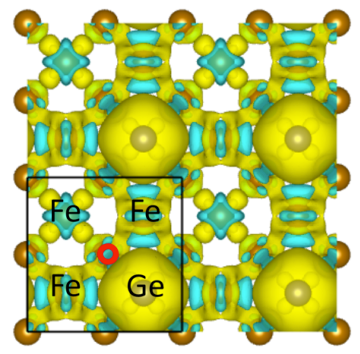
\includegraphics[width=0.45\linewidth]{Chap3/plots/Fig10b.pdf}}\label{Chap:Mg_H:fig:10b}
  \\
  \subfigure[]{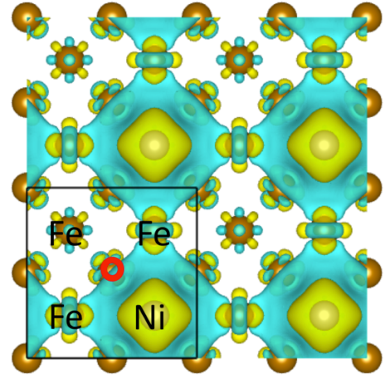
\includegraphics[width=0.45\linewidth]{Chap3/plots/Fig10c.pdf}}\label{Chap:Mg_H:fig:10c}
  \subfigure[]{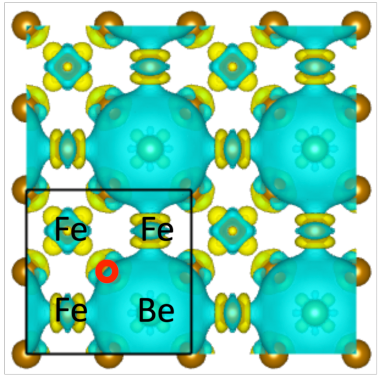
\includegraphics[width=0.45\linewidth]{Chap3/plots/Fig10d.pdf}}\label{Chap:Mg_H:fig:10d}  
\caption[Top-down views of isosurfaces of electron density difference for (2$\times$2) Fe (100) with one substitutional alloying atom in top surface layer]{Top-down views of isosurfaces of electron density difference ($\Delta \rho$ defined in Equation \ref{Chap:Mg_H:eq:chargediff}) for (2$\times$2) Fe (100) with one substitutional alloying atom in top surface layer. Surface Fe and alloy element X (X as As, Ge. Ni and Be in (a), (b), (c) and (d), respectively) are denoted. The open red circle is located at a hollow site I (Figure \ref{Chap:Mg_H:fig3} (b)) for hydrogen adsorption. The black box indicates the periodicity of a (2$\times$2) Fe (100). The yellowish isosurface is $1.0\times10^{-3}\frac{e}{bohr^3}$ corresponding to positive $\Delta \rho$ or electron accumulation after the substitutional alloying. The blue isosurface is $-1.0\times10^{-3}\frac{e}{bohr^3}$ corresponding to negative $\Delta \rho$ or electron depletion after the substitutional alloying.}
  \label{Chap:Mg_H:fig10}
\end{figure}
\endgroup

We next examined surface charge redistribution by computing and displaying the difference, $\Delta \rho$, between the electron density of a pure (2$\times$2) Fe (100)/(110) surface, $\rho_{Fe}$, and the electron density of the same surface unit cell with a substitutional X atom in the top surface layer, $\rho_{Fe+X}$, via
\begin{align}
 %(10)
\Delta \rho = \rho_{Fe+ X} - \rho_{Fe}
\label{Chap:Mg_H:eq:chargediff}
\end{align}
Results are shown in Figure \ref{Chap:Mg_H:fig9} and \ref{Chap:Mg_H:fig10} for Fe (110) and Fe (100), respectively. Yellowish contours denote positive $\Delta \rho$ or regions of electron accumulation in the surface layer, while blue contours denote negative $\Delta \rho$ or electron depletion in the surface layer. Referring to Figure \ref{Chap:Mg_H:fig9} (a), the yellowish contours surrounding the adsorbed As denote electron concentration in a shape resembling an s orbital with p-character. Figure \ref{Chap:Mg_H:fig9} (a) also shows a network of electron accumulation that encircles the As atom and flows through Fe surface atoms. This is somewhat counter-intuitive since As has five valence electrons, which is less than the eight in Fe. This electron accumulation around the As atom suggests the enhancement of both the spatial extent and electron density of the s/p orbital for the As atom compared with the pure Fe surface. When a H atom is absorbed at the hollow site near the As atom, indicated by the red circle in Figure \ref{Chap:Mg_H:fig9} (a), the electrons from the adsorbed H atom and those from the substitutional As atom should overlap, and quantum mechanics requires that they must be orthogonal to each other. This drives up the energy and leads to so-called Pauli repulsion as described by $E_{repulsive}$ in Equation \ref{Chap:Mg_H:eq:electronic}. Therefore, the s/p orbital for an As atom adsorbed on Fe (110) results in larger Pauli repulsion of the nearby H atom, making the H adsorption energy weaker relative to adsorption on a pure Fe surface. 


Similar effects were also predicted for adsorbed Ge on Fe (110), as shown in Figure \ref{Chap:Mg_H:fig9} (b), as well as Al, Si, Ga, and P ($\Delta \rho$ contours not shown). Alternatively, the electron distribution is depleted around the adsorbed Ni atom in Figure \ref{Chap:Mg_H:fig9} (c) (relative to As in Figure \ref{Chap:Mg_H:fig9} (a)) and even more so around the adsorbed Be atom in Figure \ref{Chap:Mg_H:fig9} (d). This is consistent with the observation from our high-throughput computations that neither Ni nor Be repels an H adsorbate on Fe surfaces, and the H adsorption energy in both cases is close to that of pure Fe (110). Observations for alloying elements on Fe (110) also apply to Fe (100) as shown in Figure \ref{Chap:Mg_H:fig10} (a) for As and Figure \ref{Chap:Mg_H:fig10} (b) for Ge (as well as Al, whose $\Delta \rho$ contours not shown). All of these elements have electron accumulation that resembles that for As on Fe (110) in Figure \ref{Chap:Mg_H:fig9} (a), and their corresponding H adsorption energies notably change from -0.4 eV/atom to $\sim$ -0.2 eV/atom. Alternatively, Figure \ref{Chap:Mg_H:fig10} (c) shows that Ni has only a small local electron accumulation in Fe (100) while electron density is severely depleted around Be in Figure \ref{Chap:Mg_H:fig10} (d). This is consistent with the conclusion from our high-throughput computations that H adsorption in the presence of Be and Ni on Fe (100) is not weakened.

\newpage
\begingroup
\begin{figure}[!ht]
  \centering
  \subfigure[]{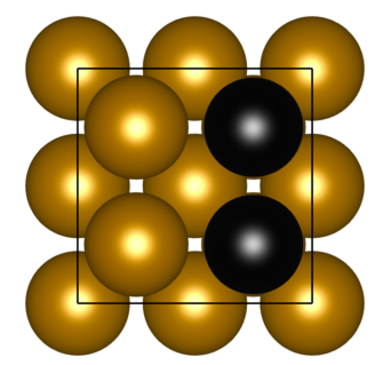
\includegraphics[width=0.3\linewidth]{Chap3/plots/Fig11a.pdf}}\label{Chap:Mg_H:fig:11a}
  \subfigure[]{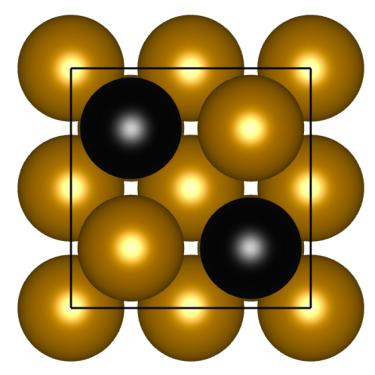
\includegraphics[width=0.3\linewidth]{Chap3/plots/Fig11b.pdf}}\label{Chap:Mg_H:fig:11b}
  \\
  \subfigure[]{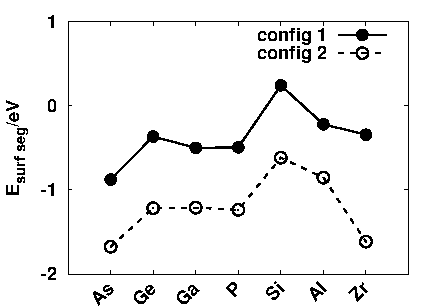
\includegraphics[width=0.5\linewidth]{Chap3/plots/Fig11c.pdf}}\label{Chap:Mg_H:fig:11c}
  \subfigure[]{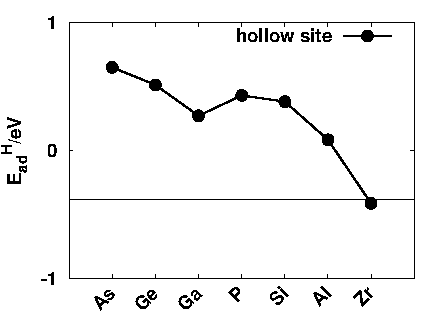
\includegraphics[width=0.5\linewidth]{Chap3/plots/Fig11d.pdf}}\label{Chap:Mg_H:fig:11d} 
\caption[Effects of 6 p-block elements on higher surface alloying coverage]{(a) and (b): two different configurations ((a) as ``config 1'' and (b) as ``config 2'')) for (2$\times$2) Fe (100) with two atoms of a generic alloying element substituting two Fe atoms in the top surface layer. (c) Segregation energies $E_{surf seg}$ defined in Eq. (7) for the second substitutional alloying atom in (2$\times$2) Fe (100) with two substitutional atoms in different final configurations ((a) and (b)). (d) H adsorption energies $E_{ad}^H$ defined in Eq. (8) on (2$\times$2) Fe (100) with two substitutional alloying atoms in the top surface layer as ``config 2'' shown in (b).}
  \label{Chap:Mg_H:fig11}
\end{figure}
\endgroup